\documentclass[12pt,a4paper]{article}
\usepackage[margin=0.72in]{geometry}
\usepackage[T1]{fontenc}
\usepackage{lmodern}
\usepackage{microtype}
\usepackage{booktabs,array,tabularx,enumitem}
\usepackage{xcolor}
\usepackage{tikz}
\usetikzlibrary{arrows.meta,positioning,shapes.geometric,fit,calc,backgrounds}
\usepackage{hyperref}
\hypersetup{colorlinks=true,linkcolor=black,urlcolor=blue}
\setlength{\parindent}{0pt}
\setlength{\parskip}{5pt}
\renewcommand{\arraystretch}{1.18}
\definecolor{lnmblue}{HTML}{1F4E79}
\definecolor{detailblue}{HTML}{D9EAF7}
\definecolor{lanegray}{HTML}{F1F3F5}
\tikzset{
  usecase/.style={ellipse,draw=black,align=center,minimum width=2.10cm,minimum height=.65cm,font=\scriptsize,fill=white},
  detailed/.style={usecase,draw=lnmblue,line width=.8pt,fill=detailblue},
  actor/.style={draw=none,align=center,font=\scriptsize},
  flow/.style={-{Stealth[length=2mm]},line width=.55pt},
  decision/.style={diamond,draw,aspect=1.65,align=center,font=\scriptsize,inner sep=1.5pt,fill=white},
  action/.style={rectangle,rounded corners=2pt,draw,align=center,font=\scriptsize,minimum width=2.25cm,minimum height=.55cm,fill=white},
  note/.style={rectangle,draw=black!60,align=left,font=\scriptsize,fill=yellow!14,inner sep=4pt}
}
\newcommand{\docheader}{%
\begin{center}\small The LNM Institute of Information Technology, Jaipur\\
Software Development Laboratory\\Course Code: CS314\end{center}\vspace{-3pt}\hrule\vspace{10pt}}
\newcommand{\stickactor}[2]{%
  \begin{scope}[shift={#1}]
  \draw[line width=.7pt] (0,0.34) circle (.10);
  \draw[line width=.7pt] (0,.24)--(0,-.13);
  \draw[line width=.7pt] (-.16,.10)--(.16,.10);
  \draw[line width=.7pt] (0,-.13)--(-.15,-.34) (0,-.13)--(.15,-.34);
  \node[font=\scriptsize,align=center,below] at (0,-.37) {#2};
\end{scope}}
\newcommand{\sectionnum}[1]{\section*{#1}}
\begin{document}

\begin{titlepage}
\centering
\vspace*{1.45cm}
{\large The LNM Institute of Information Technology, Jaipur\par}
\vspace{.35cm}
{\Large\bfseries Software Development Laboratory\par}
\vspace{.2cm}
{\large Course Code: CS314\par}
\vspace{1.5cm}
{\LARGE\bfseries Lab Assignment 3: Solution\par}
\vspace{.35cm}
{\Large Scenario, Use Case and Activity Modelling\par}
\vspace{1.35cm}
\rule{.85\textwidth}{.7pt}\par\vspace{.55cm}
{\large\bfseries Higher Studies Tracking System\par}
\vspace{.55cm}
\rule{.85\textwidth}{.7pt}\par
\vfill
\begin{tabular}{>{\bfseries}l l}
Team ID: & T070\\
Team Members: & Laxita Bhimsaria, Vaibhav Goyal, Manan Jain, Harsh Varshney\\
Roll Numbers: & 24UCS144, 24UCS145, 24UCS146, 24UCS148\\
Submitted by: & Team T070\\
Date: & 13 September 2026
\end{tabular}
\vfill
{\small This document continues the Assignment 2 requirements specification. The three detailed use cases carried forward unchanged are UC-004, UC-008 and UC-006.}\par
\end{titlepage}

\docheader
\sectionnum{25. Scenario Modelling}
The following scenarios preserve the detailed use cases defined in Assignment 2. They do not introduce functionality beyond FR-007, FR-011, FR-015--FR-017 and FR-019--FR-021.

\subsection*{25.1 Scenario: UC-004 --- Add Higher-Study Record}
\begin{tabularx}{\textwidth}{>{\bfseries}p{3.2cm} X}
Primary actor & Student/Alumnus\\
Supporting actor & Higher Studies Tracking System\\
Starting condition & The student/alumnus is authenticated, has permission to maintain the profile, and institution/programme/country information is available.\\
Main sequence & The student opens the higher-study profile and selects \emph{Add Higher-Study Record}. The system displays the required fields. The student enters institution, programme, country, admission information and other available details, then saves the record. The system validates the information, stores the record with the configured initial status (normally Draft), and confirms the save.\\
Alternative / exception & If a required value or format is invalid, the system highlights the affected fields and the student corrects them before final saving. If an institution or programme is unavailable, the student may save a draft or request its addition according to the configured process. If the session expires, the student authenticates again.\\
Expected outcome & A higher-study record exists for the student and is available for later viewing, updating and verification.\\
\end{tabularx}

\subsection*{25.2 Scenario: UC-008 --- Verify Higher-Study Record}
\begin{tabularx}{\textwidth}{>{\bfseries}p{3.2cm} X}
Primary actor & Higher Studies Coordinator\\
Supporting actors & Higher Studies Tracking System; Student/Alumnus (receives outcome)\\
Starting condition & The coordinator is authenticated and authorized, and a student higher-study record has been submitted for verification.\\
Main sequence & The coordinator opens the verification queue. The system displays submitted records. The coordinator selects one record and reviews its institution, programme, country, admission and progression details together with submission history. The coordinator selects \emph{Verify}. The system records the decision, reviewer and date, changes the record status to Verified, and informs the student.\\
Alternative / exception & If information is incomplete or incorrect, the coordinator selects \emph{Request Correction} and records a reason. The system marks the record as Correction Required and informs the student. If the record is already verified, duplicate verification is not permitted.\\
Expected outcome & The submitted record is either Verified with an audit trail or returned for correction with a visible reason.\\
\end{tabularx}

\subsection*{25.3 Scenario: UC-006 --- Update Progression}
\begin{tabularx}{\textwidth}{>{\bfseries}p{3.2cm} X}
Primary actor & Higher Studies Coordinator\\
Supporting actor & Higher Studies Tracking System\\
Starting condition & The coordinator is authenticated, authorized to update progression, and a valid higher-study record exists.\\
Main sequence & The coordinator searches for the student record. The system displays the current progression status. The coordinator selects \emph{Update Progression}, enters a new status, date and remarks, and submits the update. The system validates and stores the dated update, links it to the correct record, updates the current progression status, and displays the result.\\
Alternative / exception & If no record is found, the system shows an appropriate message. If a required value is invalid, the system asks the coordinator to correct it before the update is saved.\\
Expected outcome & The latest progression status is recorded and the dated entry remains available in the progression history.\\
\end{tabularx}

\newpage
\docheader
\sectionnum{26. UML Use Case Model}
Figure 1 models the complete initial-release system. Blue use cases are the three detailed use cases carried forward from Assignment 2.

\begin{center}
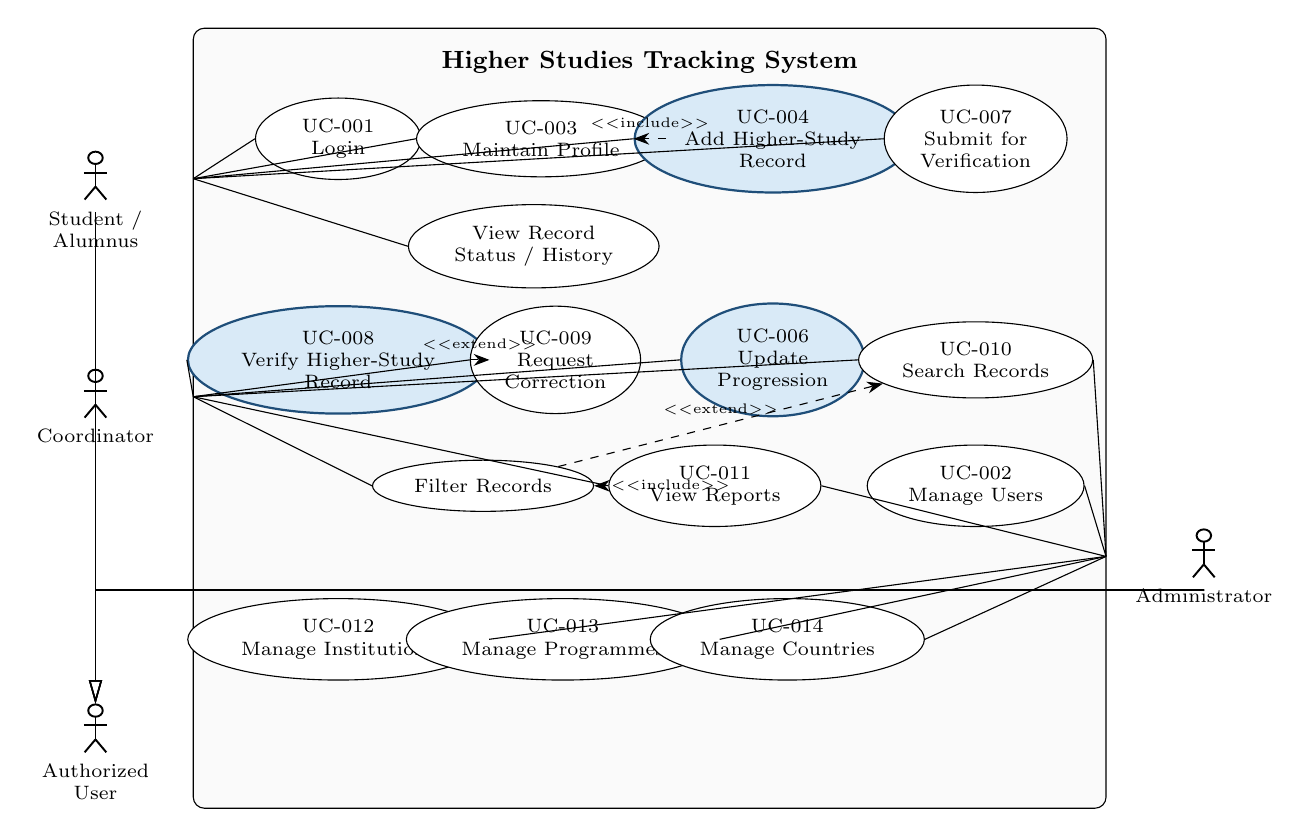
\begin{tikzpicture}[x=.92cm,y=.78cm]
  \draw[rounded corners=4pt,fill=black!2] (0,0) rectangle (12.6,12.7);
  \node[font=\small\bfseries,anchor=north] at (6.3,12.48) {Higher Studies Tracking System};
  \stickactor{(-1.35,10.25)}{Student /\\Alumnus}
  \stickactor{(-1.35,6.7)}{Coordinator}
  \stickactor{(13.95,4.1)}{Administrator}
  \stickactor{(-1.35,1.25)}{Authorized\\User}
  % use cases
  \node[usecase] (login) at (2.0,10.9) {UC-001\\Login};
  \node[usecase] (profile) at (4.8,10.9) {UC-003\\Maintain Profile};
  \node[detailed] (add) at (8.0,10.9) {UC-004\\Add Higher-Study\\Record};
  \node[usecase] (submit) at (10.8,10.9) {UC-007\\Submit for\\Verification};
  \node[usecase] (status) at (4.7,9.15) {View Record\\Status / History};
  \node[detailed] (verify) at (2.0,7.3) {UC-008\\Verify Higher-Study\\Record};
  \node[usecase] (correct) at (5.0,7.3) {UC-009\\Request\\Correction};
  \node[detailed] (progress) at (8.0,7.3) {UC-006\\Update\\Progression};
  \node[usecase] (search) at (10.8,7.3) {UC-010\\Search Records};
  \node[usecase] (filter) at (4.0,5.25) {Filter Records};
  \node[usecase] (reports) at (7.2,5.25) {UC-011\\View Reports};
  \node[usecase] (users) at (10.8,5.25) {UC-002\\Manage Users};
  \node[usecase] (institution) at (2.0,2.75) {UC-012\\Manage Institutions};
  \node[usecase] (programme) at (5.1,2.75) {UC-013\\Manage Programmes};
  \node[usecase] (country) at (8.2,2.75) {UC-014\\Manage Countries};
  % Associations
  \draw (0,10.25) -- (login.west); \draw (0,10.25) -- (profile.west); \draw (0,10.25) -- (add.west);
  \draw (0,10.25) -- (submit.west); \draw (0,10.25) -- (status.west);
  \draw (0,6.7) -- (verify.west); \draw (0,6.7) -- (correct.west); \draw (0,6.7) -- (progress.west);
  \draw (0,6.7) -- (search.west); \draw (0,6.7) -- (filter.west); \draw (0,6.7) -- (reports.west);
  \draw (12.6,4.1) -- (users.east); \draw (12.6,4.1) -- (institution.east); \draw (12.6,4.1) -- (programme.east);
  \draw (12.6,4.1) -- (country.east); \draw (12.6,4.1) -- (search.east); \draw (12.6,4.1) -- (reports.east);
  % actor generalization
  \draw[-{Triangle[open,length=3mm]},line width=.55pt] (-1.35,9.70) -- (-1.35,1.70);
  \draw[-{Triangle[open,length=3mm]},line width=.55pt] (-1.35,6.15) -- (-1.35,1.70);
  \draw[-{Triangle[open,length=3mm]},line width=.55pt] (13.95,3.55) -| (-1.35,1.70);
  % relationships
  \draw[-{Stealth[length=2mm]},dashed] (profile) -- node[midway,above,font=\tiny]{\textless\textless include\textgreater\textgreater} (add);
  \draw[-{Stealth[length=2mm]},dashed] (correct) -- node[midway,above,font=\tiny]{\textless\textless extend\textgreater\textgreater} (verify);
  \draw[-{Stealth[length=2mm]},dashed] (filter) -- node[midway,above,font=\tiny]{\textless\textless extend\textgreater\textgreater} (search);
  \draw[-{Stealth[length=2mm]},dashed] (reports) -- node[midway,right,font=\tiny]{\textless\textless include\textgreater\textgreater} (filter);
\end{tikzpicture}
\end{center}
\begin{center}\small\textbf{Figure 1:} UML Use Case Diagram for the Higher Studies Tracking System\end{center}

\textbf{Relationship rationale.} Maintaining a profile includes adding a higher-study record. Request Correction is an optional outcome that extends verification. Filtering is optional refinement of a search, and report generation includes filtering the relevant record set. Student/Alumnus, Coordinator and Administrator specialize the shared Authorized User role.

\newpage
\docheader
\sectionnum{27. UML Activity Diagrams}
Each activity diagram uses the exact preconditions, normal flow and exception flow specified in the Assignment 2 detailed use case. Swimlanes identify responsibility. There is no artificial synchronization: each carried-forward workflow is sequential, so forks/joins are not applicable.

\subsection*{27.1 UC-004 --- Add Higher-Study Record}
\begin{center}
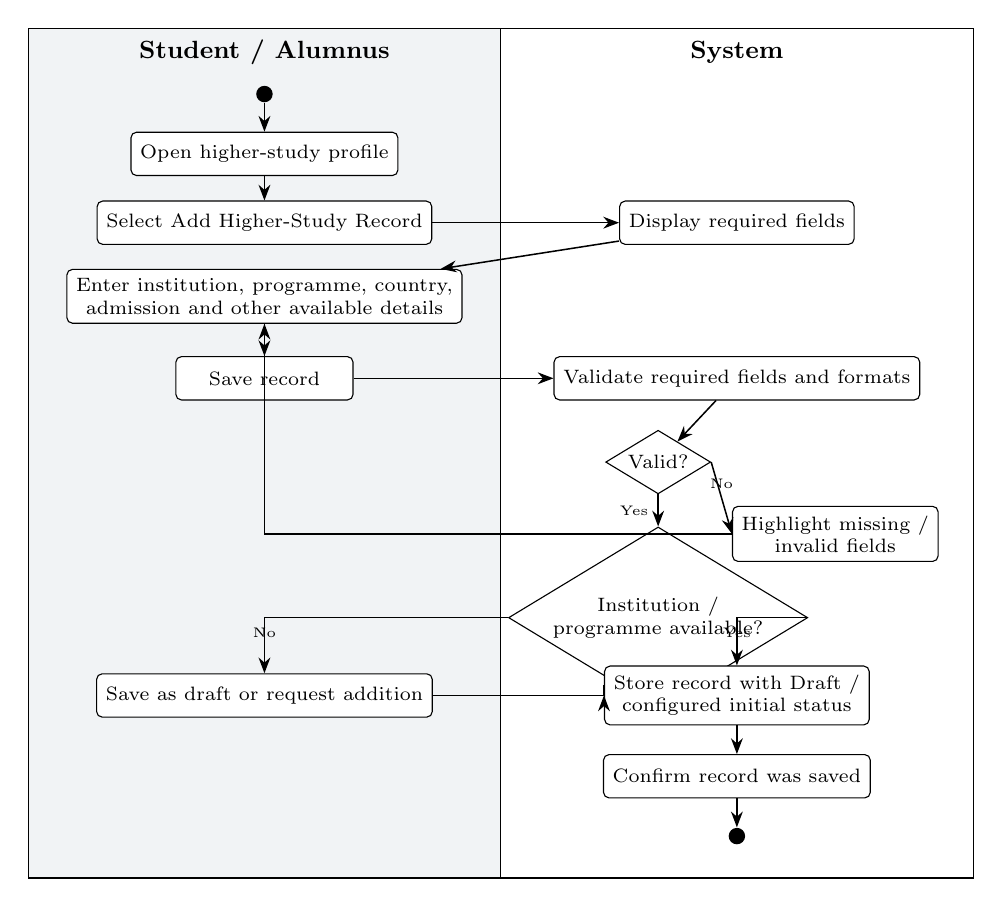
\begin{tikzpicture}[x=1cm,y=.76cm]
  \fill[lanegray] (0,0) rectangle (6.0,14.2); \draw (0,0) rectangle (12,14.2); \draw (6,0)--(6,14.2);
  \node[font=\small\bfseries] at (3,13.8) {Student / Alumnus}; \node[font=\small\bfseries] at (9,13.8) {System};
  \node[fill=black,circle,inner sep=2.1pt] (start) at (3,13.1) {};
  \node[action] (open) at (3,12.1) {Open higher-study profile};
  \node[action] (select) at (3,10.95) {Select Add Higher-Study Record};
  \node[action] (fields) at (9,10.95) {Display required fields};
  \node[action] (enter) at (3,9.72) {Enter institution, programme, country,\\admission and other available details};
  \node[action] (save) at (3,8.35) {Save record};
  \node[action] (validate) at (9,8.35) {Validate required fields and formats};
  \node[decision] (valid) at (8.0,6.95) {Valid?};
  \node[action] (error) at (10.25,5.75) {Highlight missing /\\invalid fields};
  \node[decision] (available) at (8.0,4.35) {Institution /\\programme available?};
  \node[action] (draft) at (3,3.05) {Save as draft or request addition};
  \node[action] (store) at (9,3.05) {Store record with Draft /\\configured initial status};
  \node[action] (confirm) at (9,1.70) {Confirm record was saved};
  \node[fill=black,circle,inner sep=2.1pt] (end) at (9,.70) {};
  \draw[flow] (start)--(open); \draw[flow] (open)--(select); \draw[flow] (select)--(fields); \draw[flow] (fields)--(enter); \draw[flow] (enter)--(save); \draw[flow] (save)--(validate); \draw[flow] (validate)--(valid);
  \draw[flow] (valid.east) -- node[above,font=\tiny]{No}(error.west); \draw[flow] (error.west) -| (enter.south);
  \draw[flow] (valid.south)--node[left,font=\tiny]{Yes}(available.north); \draw[flow] (available.east)-|node[below,font=\tiny]{Yes}(store.north); \draw[flow] (available.west)-|node[below,font=\tiny]{No}(draft.north); \draw[flow] (draft.east)-|(store.west);
  \draw[flow] (store)--(confirm); \draw[flow] (confirm)--(end);
\end{tikzpicture}
\end{center}
\begin{center}\small\textbf{Figure 2:} Activity Diagram --- UC-004 Add Higher-Study Record\end{center}

\newpage
\docheader
\subsection*{27.2 UC-008 --- Verify Higher-Study Record}
\begin{center}
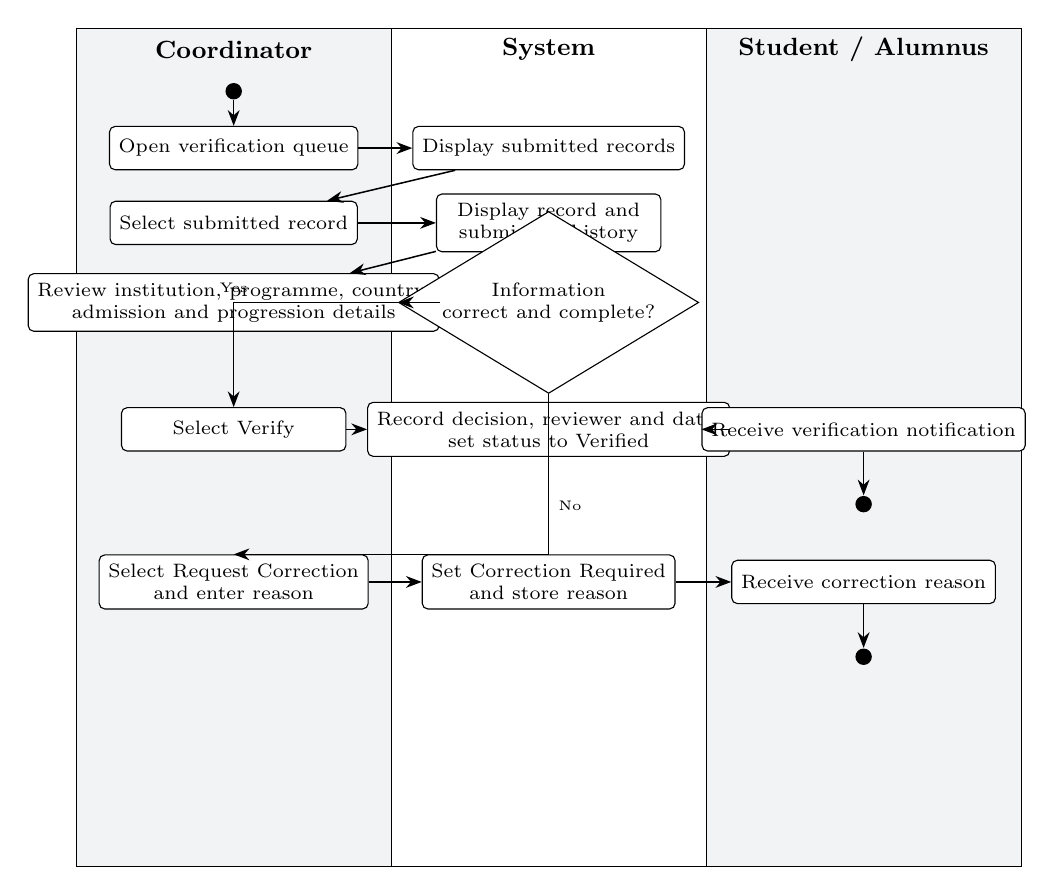
\begin{tikzpicture}[x=1cm,y=.76cm]
  \fill[lanegray] (0,0) rectangle (4,14.0); \fill[lanegray] (8,0) rectangle (12,14.0);
  \draw (0,0) rectangle (12,14.0); \draw (4,0)--(4,14.0); \draw (8,0)--(8,14.0);
  \node[font=\small\bfseries] at (2,13.65) {Coordinator}; \node[font=\small\bfseries] at (6,13.65) {System}; \node[font=\small\bfseries] at (10,13.65) {Student / Alumnus};
  \node[fill=black,circle,inner sep=2.1pt] (start) at (2,12.95) {};
  \node[action,minimum width=2.85cm] (queue) at (2,12.0) {Open verification queue};
  \node[action,minimum width=2.85cm] (list) at (6,12.0) {Display submitted records};
  \node[action,minimum width=2.85cm] (choose) at (2,10.75) {Select submitted record};
  \node[action,minimum width=2.85cm] (details) at (6,10.75) {Display record and\\submission history};
  \node[action,minimum width=2.85cm] (review) at (2,9.42) {Review institution, programme, country,\\admission and progression details};
  \node[decision] (complete) at (6,9.42) {Information\\correct and complete?};
  \node[action,minimum width=2.85cm] (verify) at (2,7.30) {Select Verify};
  \node[action,minimum width=2.85cm] (recordverify) at (6,7.30) {Record decision, reviewer and date;\\set status to Verified};
  \node[action,minimum width=2.85cm] (correct) at (2,4.75) {Select Request Correction\\and enter reason};
  \node[action,minimum width=2.85cm] (recordcorrect) at (6,4.75) {Set Correction Required\\and store reason};
  \node[action,minimum width=2.85cm] (notifyv) at (10,7.30) {Receive verification notification};
  \node[action,minimum width=2.85cm] (notifyc) at (10,4.75) {Receive correction reason};
  \node[fill=black,circle,inner sep=2.1pt] (endv) at (10,6.05) {};
  \node[fill=black,circle,inner sep=2.1pt] (endc) at (10,3.50) {};
  \draw[flow] (start)--(queue); \draw[flow] (queue)--(list); \draw[flow] (list)--(choose); \draw[flow] (choose)--(details); \draw[flow] (details)--(review); \draw[flow] (review)--(complete);
  \draw[flow] (complete.west)-|node[above,font=\tiny]{Yes}(verify.north); \draw[flow] (verify)--(recordverify); \draw[flow] (recordverify)--(notifyv); \draw[flow] (notifyv)--(endv);
  \draw[flow] (complete.south) |- node[pos=.35,right,font=\tiny]{No}(correct.north); \draw[flow] (correct)--(recordcorrect); \draw[flow] (recordcorrect)--(notifyc); \draw[flow] (notifyc)--(endc);
\end{tikzpicture}
\end{center}
\begin{center}\small\textbf{Figure 3:} Activity Diagram --- UC-008 Verify Higher-Study Record\end{center}

\newpage
\docheader
\subsection*{27.3 UC-006 --- Update Progression}
\begin{center}
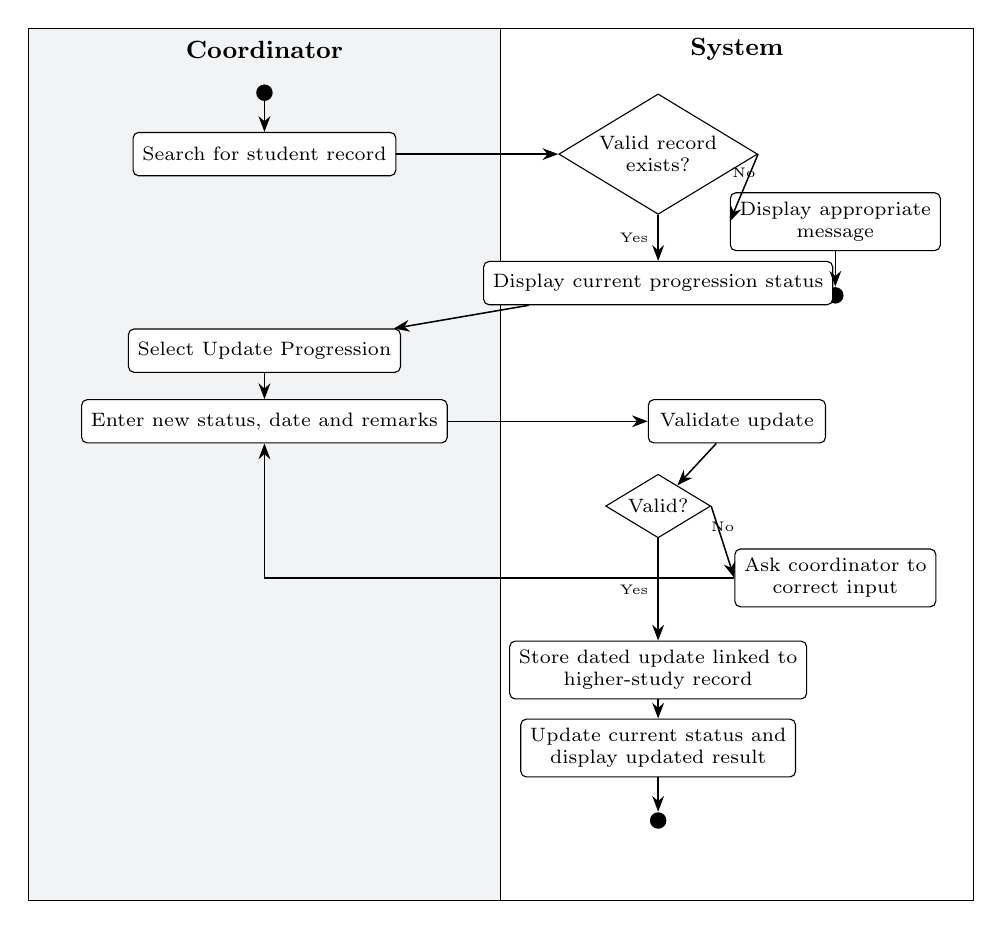
\begin{tikzpicture}[x=1cm,y=.78cm]
  \fill[lanegray] (0,0) rectangle (6,14.2); \draw (0,0) rectangle (12,14.2); \draw (6,0)--(6,14.2);
  \node[font=\small\bfseries] at (3,13.85) {Coordinator}; \node[font=\small\bfseries] at (9,13.85) {System};
  \node[fill=black,circle,inner sep=2.1pt] (start) at (3,13.15) {};
  \node[action] (search) at (3,12.15) {Search for student record};
  \node[decision] (exists) at (8.0,12.15) {Valid record\\exists?};
  \node[action] (notfound) at (10.25,11.05) {Display appropriate\\message};
  \node[fill=black,circle,inner sep=2.1pt] (endnf) at (10.25,9.85) {};
  \node[action] (current) at (8.0,10.05) {Display current progression status};
  \node[action] (select) at (3,8.95) {Select Update Progression};
  \node[action] (enter) at (3,7.80) {Enter new status, date and remarks};
  \node[action] (validate) at (9,7.80) {Validate update};
  \node[decision] (valid) at (8.0,6.42) {Valid?};
  \node[action] (error) at (10.25,5.25) {Ask coordinator to\\correct input};
  \node[action] (store) at (8.0,3.75) {Store dated update linked to\\higher-study record};
  \node[action] (update) at (8.0,2.48) {Update current status and\\display updated result};
  \node[fill=black,circle,inner sep=2.1pt] (end) at (8.0,1.30) {};
  \draw[flow] (start)--(search); \draw[flow] (search)--(exists); \draw[flow] (exists.east)--node[above,font=\tiny]{No}(notfound.west); \draw[flow] (notfound)--(endnf);
  \draw[flow] (exists.south)--node[left,font=\tiny]{Yes}(current.north); \draw[flow] (current)--(select); \draw[flow] (select)--(enter); \draw[flow] (enter)--(validate); \draw[flow] (validate)--(valid);
  \draw[flow] (valid.east)--node[above,font=\tiny]{No}(error.west); \draw[flow] (error.west)-|(enter.south);
  \draw[flow] (valid.south)--node[left,font=\tiny]{Yes}(store.north); \draw[flow] (store)--(update); \draw[flow] (update)--(end);
\end{tikzpicture}
\end{center}
\begin{center}\small\textbf{Figure 4:} Activity Diagram --- UC-006 Update Progression\end{center}

\newpage
\docheader
\sectionnum{28. Consistency and Traceability}
\begin{tabularx}{\textwidth}{>{\bfseries}p{2.0cm} p{3.4cm} X}
Detailed use case & Assignment 2 requirement links & Assignment 3 artefacts\\ \midrule
UC-004 Add Higher-Study Record & FR-007 Update Profile; FR-008 Institution Details; FR-009 Programme Details; FR-010 Country Details; BR-007 & Scenario 25.1; highlighted use case in Figure 1; Activity Diagram in Figure 2\\
UC-008 Verify Higher-Study Record & FR-019 Submit for Verification; FR-020 Verify Record; FR-021 Request Correction; FR-022 Record Status; BR-004 & Scenario 25.2; highlighted use case in Figure 1; Activity Diagram in Figure 3\\
UC-006 Update Progression & FR-015 Progression Status; FR-016 Progress Update; FR-017 Progress History; FR-018 Completion Status; BR-008 & Scenario 25.3; highlighted use case in Figure 1; Activity Diagram in Figure 4\\
\end{tabularx}

\vspace{10pt}
\textbf{Modelling consistency statement.} The use case model, scenarios and activity diagrams use the same actors, conditions, actions, alternate paths and outcomes as the three Assignment 2 detailed use cases. The model only organizes existing requirements; it does not add new system functionality.

\sectionnum{29. Individual Contribution}
\begin{tabularx}{\textwidth}{>{\bfseries}p{3.4cm} X}
Laxita Bhimsaria & Scenario drafting and consistency review for UC-004; review of the complete use case model.\\
Vaibhav Goyal & Scenario drafting and activity modelling for UC-008.\\
Manan Jain & UML use case diagram; activity modelling for UC-006; requirements-to-model traceability.\\
Harsh Varshney & Activity modelling for UC-004; formatting, verification and final compilation.\\
\end{tabularx}

\vfill
\section*{AI Usage Policy --- Student Declaration}
AI tools may be used as supporting tools for this assignment. The team is responsible for the correctness, consistency and understanding of all submitted scenarios and UML models.
\begin{itemize}[leftmargin=1.4em,itemsep=2pt]
\item We have disclosed the use of AI tools, if any.
\item AI-generated suggestions have been reviewed, verified and adapted by the team.
\item We understand and can explain the submitted scenarios, use case diagram and activity diagrams.
\item We have verified that the UML models are consistent with the project requirements, use cases and scope.
\item The final submission represents our team's understanding and modelling decisions.
\end{itemize}
\begin{tabular}{>{\bfseries}l l}
AI Tool(s) Used: & ChatGPT\\
Purpose of AI Use: & Supporting organisation, UML modelling and document drafting; reviewed by the team.\\
Team ID: & T070\\
Team Representative: & Laxita Bhimsaria\\
Date: & 13 September 2026
\end{tabular}

\end{document}
